\documentclass[12pt,a4paper]{extarticle}
\usepackage[utf8]{inputenc}
\usepackage[T5]{fontenc}
\usepackage{geometry}
\geometry{a4paper, left=1.5cm, right=1cm, top=1.5cm, bottom=1.5cm, headheight=20pt, headsep=15pt, footskip=28pt}
\usepackage{enumitem}
\usepackage{amsmath}
\usepackage{diagbox}
\usepackage[most]{tcolorbox}
\newcommand{\khongxacdinh}{\text{KXĐ}}
\newcommand{\blackbox}[1]{\texorpdfstring{\fcolorbox{black}{black}{\textcolor{white}{#1}}}{#1}}
\usepackage{tikz}
\definecolor{bookmagenta}{RGB}{58,90,172}
\definecolor{book}{RGB}{58,90,172}
\newtcolorbox{formulaBox}{colback=gray!5,colframe=bookmagenta,boxrule=0.8pt,arc=2mm}
\usetikzlibrary{patterns, patterns.meta} % Thêm patterns.meta vào đây
% Gọi package nằm trong thư mục con template
\usepackage{../template/mngocbox}

\begin{document}

% Sử dụng ngoặc vuông [...] để thay đổi linh hoạt các thông số
\makeheadbox[headerright={Tổng ôn 10-11},chude={CHỦ ĐỀ 03},tieude={Hệ thức lượng trong tam giác},dinhdang={Đại số},lop={12 },gv={Nguyễn Lê Minh Ngọc}]

\vspace{2em}
\makeheading{I}{Tóm tắt lý thuyết}
\section{Giá trị lượng giác của một góc}
Trong mặt phẳng $Oxy$ nửa đường tròn tâm O, bán kính $R=1$ nằm phía trên trục hoành như hình dưới đây được gọi là nửa đường tròn đơn vị.\\
\vspace{1cm}

Cho trước một góc $\alpha$, $0^\circ \le \alpha \le 180^\circ$. Khi đó có duy nhất điểm $M(x_0; y_0)$ trên nửa đường tròn đơn vị nói trên để $xOM = \alpha$.
\begin{center}
    \begin{minipage}{0.48\textwidth}
        \centering
        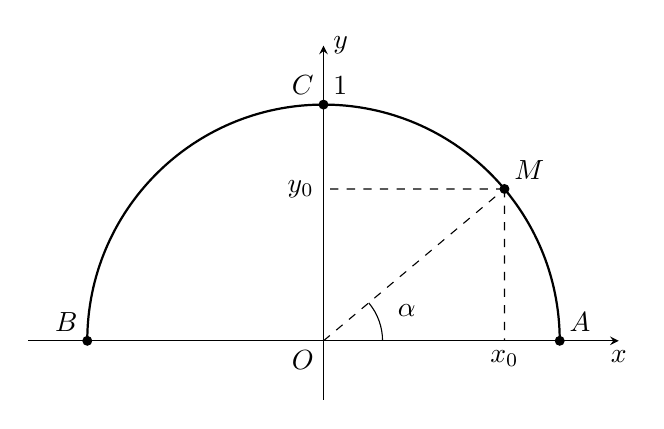
\begin{tikzpicture}[scale=1.5, >=stealth]
            % Trục tọa độ
            \draw[->] (-2.5, 0) -- (2.5, 0) node[below] {$x$};
            \draw[->] (0, -0.5) -- (0, 2.5) node[right] {$y$};
            \node[below left] at (0, 0) {$O$};
            
            % Nửa đường tròn đơn vị
            \draw[thick] (2, 0) arc (0:180:2);
            
            % Các điểm mốc A, B, C và nhãn 1
            \fill (2, 0) circle (1.2pt) node[above right] {$A$};
            \fill (-2, 0) circle (1.2pt) node[above left] {$B$};
            \fill (0, 2) circle (1.2pt) node[above left] {$C$};
            \node[above right] at (0, 2) {$1$};
            
            % Điểm M ở góc nhọn (ví dụ 40 độ)
            \coordinate (M) at (40:2);
            \fill (M) circle (1.2pt) node[above right] {$M$};
            
            % Nối O với M
            \draw[dashed] (0, 0) -- (M);
            
            % Đường hạ vuông góc xuống Ox và Oy
            \draw[dashed] (M) -- ({2*cos(40)}, 0) node[below] {$x_0$};
            \draw[dashed] (M) -- (0, {2*sin(40)}) node[left] {$y_0$};
            
            % Cung biểu diễn góc alpha
            \draw (0.5, 0) arc (0:40:0.5);
            \node at (20:0.75) {$\alpha$};
        \end{tikzpicture}
        
        \vspace{0.3cm}
        $\alpha < 90^\circ$
    \end{minipage}
    \hfill
    \begin{minipage}{0.48\textwidth}
        \centering
        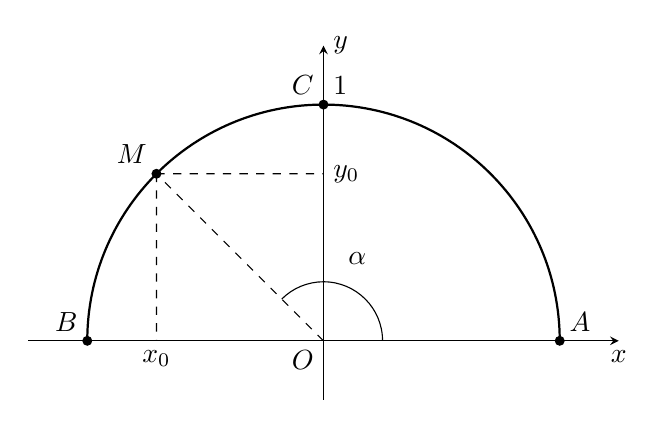
\begin{tikzpicture}[scale=1.5, >=stealth]
            % Trục tọa độ
            \draw[->] (-2.5, 0) -- (2.5, 0) node[below] {$x$};
            \draw[->] (0, -0.5) -- (0, 2.5) node[right] {$y$};
            \node[below left] at (0, 0) {$O$};
            
            % Nửa đường tròn đơn vị
            \draw[thick] (2, 0) arc (0:180:2);
            
            % Các điểm mốc A, B, C và nhãn 1
            \fill (2, 0) circle (1.2pt) node[above right] {$A$};
            \fill (-2, 0) circle (1.2pt) node[above left] {$B$};
            \fill (0, 2) circle (1.2pt) node[above left] {$C$};
            \node[above right] at (0, 2) {$1$};
            
            % Điểm M ở góc tù (ví dụ 135 độ)
            \coordinate (M) at (135:2);
            \fill (M) circle (1.2pt) node[above left] {$M$};
            
            % Nối O với M
            \draw[dashed] (0, 0) -- (M);
            
            % Đường hạ vuông góc xuống Ox và Oy
            \draw[dashed] (M) -- ({2*cos(135)}, 0) node[below] {$x_0$};
            \draw[dashed] (M) -- (0, {2*sin(135)}) node[right] {$y_0$};
            
            % Cung biểu diễn góc alpha
            \draw (0.5, 0) arc (0:135:0.5);
            \node at (67.5:0.75) {$\alpha$};
        \end{tikzpicture}
        
        \vspace{0.3cm}
        $\alpha > 90^\circ$
    \end{minipage}
\end{center}
\vspace{0.5cm}
Với mỗi góc $\alpha$ ($0^\circ \le \alpha \le 180^\circ$) gọi $M(x_0; y_0)$ là điểm trên nửa đường tròn đơn vị sao cho $xOM = \alpha$. Khi đó:
\begin{itemize}
    \item $\sin$ của góc $\alpha$ là tung độ $y_0$ của điểm $M$ được kí hiệu là $\sin \alpha$
    \item côsin của góc $\alpha$ là hoành độ $x_0$ của điểm $M$ được kí hiệu là $\cos \alpha$
    \item Khi $\alpha \ne 90^\circ$ (hay là $x_0 \ne 0$), tang của $\alpha$ là $\dfrac{y_0}{x_0}$ được kí hiệu là $\tan \alpha$
    \item Khi $\alpha \ne 0^\circ$ và $\alpha \ne 180^\circ$ (hay là $y_0 \ne 0$) côtang của $\alpha$ là $\dfrac{x_0}{y_0}$ được kí hiệu là $\cot \alpha$.
\end{itemize}
Từ định nghĩa trên ta có:
\[
\tan\alpha = \frac{\sin\alpha}{\cos\alpha} \ (\alpha \ne 90^\circ); \quad \cot\alpha = \frac{\cos\alpha}{\sin\alpha} \ (\alpha \ne 0^\circ \text{ và } \alpha \ne 180^\circ); \quad \tan\alpha = \frac{1}{\cot\alpha} \ (\alpha \notin \{0^\circ; 90^\circ; 180^\circ\})
\]
Sau đây là bảng giá trị lượng giác (GTLG) của một số góc đặc biệt nên nhớ.
\begin{center}
\renewcommand{\arraystretch}{2.2} % Tăng khoảng cách dòng trong bảng cho dễ nhìn phân số
\begin{tabular}{|c|c|c|c|c|c|c|}
    \hline
    \diagbox{\raisebox{-1ex}{\textbf{GTLG}}}{\raisebox{1ex}{$\alpha$}} & $0^\circ$ & $30^\circ$ & $45^\circ$ & $60^\circ$ & $90^\circ$ & $180^\circ$ \\
    \hline
    $\sin\alpha$ & $0$ & $\dfrac{1}{2}$ & $\dfrac{\sqrt{2}}{2}$ & $\dfrac{\sqrt{3}}{2}$ & $1$ & $0$ \\
    \hline
    $\cos\alpha$ & $1$ & $\dfrac{\sqrt{3}}{2}$ & $\dfrac{\sqrt{2}}{2}$ & $\dfrac{1}{2}$ & $0$ & $-1$ \\
    \hline
    $\tan\alpha$ & $0$ & $\dfrac{\sqrt{3}}{3}$ & $1$ & $\sqrt{3}$ & $\khongxacdinh$ & $0$ \\
    \hline
    $\cot\alpha$ & $\khongxacdinh$ & $\sqrt{3}$ & $1$ & $\dfrac{\sqrt{3}}{3}$ & $0$ & $\khongxacdinh$ \\
    \hline
\end{tabular}
\end{center}
\vspace{0.5cm}
\subsection*{\blackbox{2} \ Mối quan hệ giữa các giá trị lượng giác}
\begin{itemize}
    \item \textbf{Hai góc bù nhau:}
    \[\begin{aligned}
        \sin(180^\circ - \alpha) &= \sin\alpha \\
        \cos(180^\circ - \alpha) &= -\cos\alpha \\
        \tan(180^\circ - \alpha) &= -\tan\alpha \\
        \cot(180^\circ - \alpha) &= -\cot\alpha
    \end{aligned}\]
    
    \item \textbf{Hai góc phụ nhau:}
    \[\begin{aligned}
        \sin(90^\circ - \alpha) &= \cos\alpha \\
        \cos(90^\circ - \alpha) &= \sin\alpha \\
        \tan(90^\circ - \alpha) &= \cot\alpha \\
        \cot(90^\circ - \alpha) &= \tan\alpha
    \end{aligned}\]
     \item \textbf{Hai cung đối nhau: ($\alpha$ và $-\alpha$)}
    \[\begin{aligned}
        \cos(-\alpha) &= \cos\alpha \\
        \sin(-\alpha) &= -\sin\alpha \\
        \tan(-\alpha) &= -\tan\alpha \\
        \cot(-\alpha) &= -\cot\alpha
    \end{aligned}\]
    \item \textbf{Hai cung hơn, kém $\pi$: ($\alpha$ và $\pi + \alpha$)}
    \[\begin{aligned}
        \sin(\pi + \alpha) &= -\sin\alpha \\
        \cos(\pi + \alpha) &= -\cos\alpha \\
        \tan(\pi + \alpha) &= \tan\alpha \\
        \cot(\pi + \alpha) &= \cot\alpha
    \end{aligned}\]
    \item \textbf{Cung hơn kém $\dfrac{\pi}{2}$:}
    \[\begin{aligned}
        \cos\left(\frac{\pi}{2} + x\right) &= -\sin x; \quad \sin\left(\frac{\pi}{2} + x\right) = \cos x;
    \end{aligned}\]
\end{itemize}
\subsection*{\blackbox{3} \ Các hệ thức lượng giác cơ bản}
\begin{center}
\renewcommand{\arraystretch}{2}
\begin{tabular}{p{0.48\textwidth} p{0.48\textwidth}}
    $\bullet$ $\tan\alpha = \dfrac{\sin\alpha}{\cos\alpha} \ (\alpha \ne 90^\circ)$ & 
    $\bullet$ $\cot\alpha = \dfrac{\cos\alpha}{\sin\alpha} \ (\alpha \ne 0^\circ; 180^\circ)$ \\
    
    $\bullet$ $\tan\alpha \cdot \cot\alpha = 1 \ (\alpha \ne 0^\circ; 90^\circ; 180^\circ)$ & 
    $\bullet$ $\sin^2\alpha + \cos^2\alpha = 1$ \\
    
    $\bullet$ $1 + \tan^2\alpha = \dfrac{1}{\cos^2\alpha} \ (\alpha \ne 90^\circ)$ & 
    $\bullet$ $1 + \cot^2\alpha = \dfrac{1}{\sin^2\alpha} \ (\alpha \ne 0^\circ; 180^\circ)$
\end{tabular}
\end{center}
\subsection*{\blackbox{4} Công thức cộng}
\[\begin{aligned}
    \sin(a \pm b) &= \sin a \cdot \cos b \pm \cos a \cdot \sin b \\
    \cos(a \pm b) &= \cos a \cdot \cos b \mp \sin a \cdot \sin b \\
    \tan(a \pm b) &= \frac{\tan a \pm \tan b}{1 \mp \tan a \cdot \tan b}
\end{aligned}\]
\subsection*{\blackbox{5} Công thức nhân đôi}
\[\begin{aligned}
    \sin 2a &= 2 \sin a \cos a \\
    \cos 2a &= \cos^2 a - \sin^2 a = 2 \cos^2 a - 1 = 1 - 2 \sin^2 a \\
    \tan 2a &= \frac{2 \tan a}{1 - \tan^2 a}
\end{aligned}\]
\subsection*{\blackbox{6} Công thức nhân ba}
\[\begin{aligned}
    \sin 3a &= 3 \sin a - 4 \sin^3 a \\
    \cos 3a &= 4 \cos^3 a - 3 \cos a \\
    \tan 3a &= \frac{3 \tan a - \tan^3 a}{1 - 3 \tan^2 a}
\end{aligned}\]
\subsection*{\blackbox{7} Công thức hạ bậc}
\begin{center}
\renewcommand{\arraystretch}{2.5}
\begin{tabular}{p{0.48\textwidth} p{0.48\textwidth}}
    $\sin^2 a = \dfrac{1 - \cos 2a}{2}$ & 
    $\cos^2 a = \dfrac{1 + \cos 2a}{2}$ \\
    
    $\sin^3 a = \dfrac{3 \sin a - \sin 3a}{4}$ & 
    $\cos^3 a = \dfrac{3 \cos a + \cos 3a}{4}$
\end{tabular}
\end{center}
\subsection*{\blackbox{8} Công thức hạ bậc}
\[\begin{aligned}
    \cos a + \cos b &= 2 \cos \frac{a+b}{2} \cos \frac{a-b}{2} \\
    \cos a - \cos b &= -2 \sin \frac{a+b}{2} \sin \frac{a-b}{2} \\
    \sin a + \sin b &= 2 \sin \frac{a+b}{2} \cos \frac{a-b}{2} \\
    \sin a - \sin b &= 2 \cos \frac{a+b}{2} \sin \frac{a-b}{2}
\end{aligned}\]
\subsection*{\blackbox{9} Công thức biến đổi tích thành tổng}
\[\begin{aligned}
    \cos a \cdot \cos b &= \frac{1}{2} \big[ \cos(a+b) + \cos(a-b) \big] \\
    \sin a \cdot \sin b &= -\frac{1}{2} \big[ \cos(a+b) - \cos(a-b) \big] \\
    \sin a \cdot \cos b &= \frac{1}{2} \big[ \sin(a+b) + \sin(a-b) \big]
\end{aligned}\]
\subsection*{\blackbox{10} Giải phương trình lượng giác}
\[\begin{aligned}
    \sin u = \sin v &\Leftrightarrow \begin{cases} u = v + k2\pi \\ u = \pi - v + k2\pi \end{cases} \\[1ex]
    \cos u = \cos v &\Leftrightarrow \begin{cases} u = v + k2\pi \\ u = -v + k2\pi \end{cases} \\[1ex]
    \tan u = \tan v &\Leftrightarrow u = v + k\pi \\
    \cot u = \cot v &\Leftrightarrow u = v + k\pi
\end{aligned}\]
\subsection*{\textit{Trường hợp đặc biệt}}
\begin{center}
\renewcommand{\arraystretch}{2.2}
\begin{tabular}{l | l}
    $\sin u = 0 \Leftrightarrow u = k\pi$ & $\cos u = 0 \Leftrightarrow u = \dfrac{\pi}{2} + k\pi$ \\
    
    $\sin u = 1 \Leftrightarrow u = \dfrac{\pi}{2} + k2\pi$ & $\cos u = 1 \Leftrightarrow u = k2\pi$ \\
    
    $\sin u = -1 \Leftrightarrow u = -\dfrac{\pi}{2} + k2\pi$ \qquad & $\cos u = -1 \Leftrightarrow u = \pi + k2\pi$
\end{tabular}
\end{center}
\subsection*{\textcolor{bookmagenta}{11 Định lý cosin}}
\begin{formulaBox}
Cho tam giác $ABC$ có $BC = a, CA = b, AB = c$. Khi đó:
\[\begin{aligned}
    a^2 &= b^2 + c^2 - 2bc \cos A \\
    b^2 &= c^2 + a^2 - 2ca \cos B \\
    c^2 &= a^2 + b^2 - 2ab \cos C
\end{aligned}\]
\end{formulaBox}
\subsection*{\textcolor{bookmagenta}{12 Định lý sin}}
\begin{formulaBox}
Cho tam giác $ABC$ có $BC = a, CA = b, AB = c$ và bán kính đường tròn ngoại tiếp là $R$.
Khi đó: $\dfrac{a}{\sin A} = \dfrac{b}{\sin B} = \dfrac{c}{\sin C} = 2R$.
\end{formulaBox}
\vspace{0.5cm}
\subsection*{\textcolor{bookmagenta}{13. GIẢI TAM GIÁC. DIỆN TÍCH TAM GIÁC}}
\subsubsection*{\textcolor{bookmagenta}{Công thức tính diện tích tam giác}}
\begin{formulaBox}
Cho tam giác $ABC$ có $BC = a, CA = b, AB = c$. Khi đó, diện tích $S$ của tam giác $ABC$ là:
\[
S = \frac{1}{2} bc \sin A = \frac{1}{2} ca \sin B = \frac{1}{2} ab \sin C
\]
\end{formulaBox}
\subsubsection*{\textcolor{bookmagenta}{Công thức Heron để tính diện tích tam giác}}
\begin{formulaBox}
Cho tam giác $ABC$ có $BC = a, CA = b, AB = c, p = \dfrac{a+b+c}{2}$. Khi đó, diện tích $S$ của tam giác $ABC$ là:
\[
S = \sqrt{p(p-a)(p-b)(p-c)}
\]
\end{formulaBox}
\subsubsection*{\textcolor{bookmagenta}{Công thức tính bán kính đường tròn ngoại tiếp}}
\begin{formulaBox}
Cho tam giác $ABC$ có $BC = a, CA = b, AB = c$. Khi đó, bán kính đường tròn ngoại tiếp $R$ của tam giác $ABC$ là:
\[
R = \frac{a}{2\sin A} = \frac{b}{2\sin B} = \frac{c}{2\sin C}, \quad R = \frac{abc}{4S}
\]
\end{formulaBox}
\subsubsection*{\textcolor{bookmagenta}{Công thức tính bán kính đường tròn nội tiếp}}
\begin{formulaBox}
Cho tam giác $ABC$ có $BC = a, CA = b, AB = c$. Khi đó, bán kính đường tròn nội tiếp $r$ của tam giác $ABC$ là:
\[
r = \frac{S}{p}
\]
\end{formulaBox}
\subsubsection*{\textcolor{bookmagenta}{Công thức độ dài đường trung tuyến}}
\begin{formulaBox}
Cho tam giác $ABC$ có $BC = a, CA = b, AB = c$ với $m_a, m_b, m_c$ là các độ dài đường trung tuyến lần lượt xuất phát từ các đỉnh $A, B, C$.
\[
m_a^2 = \frac{b^2+c^2}{2} - \frac{a^2}{4}, \quad m_b^2 = \frac{a^2+c^2}{2} - \frac{b^2}{4}, \quad m_c^2 = \frac{a^2+b^2}{2} - \frac{c^2}{4}
\]
\end{formulaBox}
\subsubsection*{\textcolor{bookmagenta}{Công thức tính độ dài đường phân giác trong}}
\begin{formulaBox}
Cho tam giác $ABC$ có $BC = a, CA = b, AB = c$ với $l_a, l_b, l_c$ là các độ dài đường phân giác trong lần lượt xuất phát từ các đỉnh $A, B, C$.
\[
l_a^2 = bc \left( 1 - \frac{a^2}{(b+c)^2} \right), \quad l_b^2 = ac \left( 1 - \frac{b^2}{(a+c)^2} \right), \quad l_c^2 = ab \left( 1 - \frac{c^2}{(a+b)^2} \right)
\]
\end{formulaBox}

\makeheading{II}{Bài tập vận dụng}
\begin{enumerate}
    % Câu 1 (Gốc: A3)
    \item Cho $\triangle ABC$ có $BC = 12, AC = 15$, góc $\hat{C} = 60^\circ$. Khi đó độ dài cạnh $AB$ là:
    
    \textcolor{book}{A.} $AB = 6\sqrt{7}$. \hspace{1cm} \textcolor{book}{B.} $AB = 3\sqrt{7}$. \hspace{1cm} \textcolor{book}{C.} $AB = 6\sqrt{21}$. \hspace{1cm} \textcolor{book}{D.} $AB = 3\sqrt{21}$.
    % Câu 2 (Gốc: B1)
    \item Cho bốn góc (trên một đường tròn lượng giác): $\alpha = -\frac{5\pi}{6}, \beta = \frac{\pi}{3}, \gamma = \frac{25\pi}{3}, \delta = \frac{19\pi}{6}$. Các góc nào có tia cuối trùng nhau?
    
    \textcolor{book}{A.} $\alpha$ và $\beta; \gamma$ và $\delta$. \hspace{1cm} \textcolor{book}{B.} $\beta, \gamma, \delta$. \hspace{1cm} \textcolor{book}{C.} $\beta$ và $\gamma; \alpha$ và $\delta$. \hspace{1cm} \textcolor{book}{D.} $\alpha, \beta, \gamma$.
    % Câu 3 (Gốc: A8)
    \item Các nhà khảo cổ học tìm được một mảnh chiếc đĩa cổ hình tròn bị vỡ. Để xác định đường kính của chiếc đĩa, họ lấy ba điểm trên vành đĩa và tiến hành đo đạc thu được kết quả như sau: $BC \approx 28,5$ cm, $\widehat{BAC} \approx 120^\circ$. Tính đường kính của chiếc đĩa theo đơn vị xăng-ti-mét (làm tròn kết quả đến hàng đơn vị).
    
    \begin{center}
        \centering
        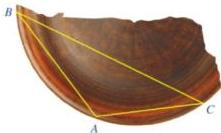
\includegraphics[width=0.4\textwidth]{img-2.jpeg}
    \end{center}
    \textcolor{book}{$\Rightarrow$} Đáp số: \dots\dots\dots\dots
    % Câu 4 (Gốc: B6)
    \item Cho tam giác $ABC$. Khẳng định nào sau đây sai:
    
    \textcolor{book}{A.} $\sin \frac{A+C}{2} = \cos \frac{B}{2}$. \hspace{1.2cm} \textcolor{book}{B.} $\cos \frac{A+C}{2} = \sin \frac{B}{2}$. \\
    \textcolor{book}{C.} $\sin(A+B) = \sin C$. \hspace{1.5cm} \textcolor{book}{D.} $\cos(A+B) = \cos C$.
    % Câu 5 (Gốc: A1)
    \item Điểm $M\left(-\frac{3}{5}; \frac{4}{5}\right)$ là điểm trên đường tròn lượng giác, biểu diễn cho góc lượng giác có số đo $\alpha$. Tìm khẳng định đúng.
    
    \textcolor{book}{A.} $\cos \alpha = -\frac{3}{5}$. \hspace{1cm} \textcolor{book}{B.} $\cos \alpha = -\frac{4}{5}$. \hspace{1cm} \textcolor{book}{C.} $\cos \alpha = \frac{3}{5}$. \hspace{1cm} \textcolor{book}{D.} $\cos \alpha = \frac{4}{5}$.
    % Câu 6 (Gốc: B10)
    \item Một chiếc quạt trần năm cánh quay với tốc độ 175 vòng trong một phút. Chọn chiều quay của quạt là chiều dương.
    \begin{enumerate}
        \item Sau 5 giây, cánh quạt quay được một góc có số đo bao nhiêu radian?
        \item Sau thời gian bao lâu cánh quạt quay được một góc có số đo $42\pi$?
    \end{enumerate}
    \textcolor{book}{$\Rightarrow$} Đáp số: \dots\dots\dots\dots
    % Câu 7 (Gốc: A6)
    \item Để đo khoảng cách từ vị trí $A$ đến vị trí $B$ ở hai bên bờ một cái ao, bạn An đi dọc bờ ao từ vị trí $A$ đến vị trí $C$ và tiến hành đo các góc $BAC, BCA$. Biết $AC = 25$ m, $\widehat{BAC} = 59,95^\circ$, $\widehat{BCA} = 82,15^\circ$. Hỏi khoảng cách từ vị trí $A$ đến vị trí $B$ là bao nhiêu mét (làm tròn kết quả đến hàng đơn vị)?
    
    \begin{center}
        \centering
        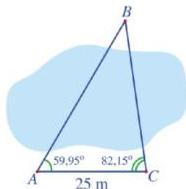
\includegraphics[width=0.4\textwidth]{img-0.jpeg}
    \end{center}
    \textcolor{book}{$\Rightarrow$} Đáp số: \dots\dots\dots\dots
    % Câu 8 (Gốc: B4)
    \item Cho biết $\sin \alpha \cdot \cos \alpha = -\frac{1}{4}$. Thì $\tan^2 \alpha + \cot^2 \alpha$ bằng
    
    \textcolor{book}{A.} 16. \hspace{1cm} \textcolor{book}{B.} 18. \hspace{1cm} \textcolor{book}{C.} 14. \hspace{1cm} \textcolor{book}{D.} 12.
    % Câu 9 (Gốc: B11)
    \item Trong chặng đua nước rút, bánh xe của một vận động viên đua xe đạp quay được 30 vòng trong 8 giây. Chọn chiều quay của bánh xe là chiều dương. Xét van V của bánh xe.
    
    \begin{center}
        \centering
        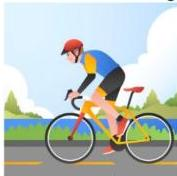
\includegraphics[width=0.3\textwidth]{img-8.jpeg}
    \end{center}
    \begin{enumerate}
        \item Sau 1 phút, van V đó quay được một góc có số đo bao nhiêu radian?
        \item Biết rằng bán kính của bánh xe là 35 cm. Độ dài quãng đường mà vận động viên đua xe đạp đã đi được trong 1 phút là bao nhiêu mét?
    \end{enumerate}
    \textcolor{book}{$\Rightarrow$} Đáp số: \dots\dots\dots\dots
    % Câu 10 (Gốc: A10)
    \item Để tính khoảng cách giữa hai địa điểm A và B mà ta không thể đi trực tiếp từ A đến B (hai địa điểm nằm ở hai bên bờ một hồ nước, một đầm lầy, ...), người ta tiến hành như sau: Chọn một địa điểm C sao cho ta đo được các khoảng cách AC, CB và góc ACB. Sau khi đo, ta nhận được: AC = 1 km, CB = 800 m và ACB = 105°. Tính khoảng cách AB (làm tròn kết quả đến hàng phần mười theo đơn vị mét).
    
    \begin{center}
        \centering
        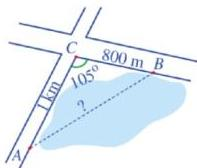
\includegraphics[width=0.4\textwidth]{img-4.jpeg}
    \end{center}
    \textcolor{book}{$\Rightarrow$} Đáp số: \dots\dots\dots\dots
    % Câu 11 (Gốc: B9)
    \item Hải lí là một đơn vị chiều dài hàng hải, được tính bằng độ dài một cung chắn một góc $\alpha = \left(\frac{1}{60}\right)^\circ$ của đường kính tuyến. Đổi số đo $\alpha$ sang radian và cho biết một hải lí bằng khoảng bao nhiêu kilômét, biết bán kính trung bình của Trái Đất là 6 371 km. Làm tròn kết quả đến hàng phần trăm.
    
    \begin{center}
        \centering
        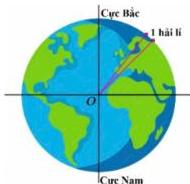
\includegraphics[width=0.3\textwidth]{img-7.jpeg}
    \end{center}
    \textcolor{book}{$\Rightarrow$} Đáp số: \dots\dots\dots\dots
    % Câu 12 (Gốc: A5)
    \item Cho $\triangle ABC$ có $\hat{B} = 45^\circ, AC = 28, BC = 25$. Số đo của góc $A$ gần bằng
    
    \textcolor{book}{A.} $39,1^\circ$. \hspace{1cm} \textcolor{book}{B.} $40,2^\circ$. \hspace{1cm} \textcolor{book}{C.} $39,2^\circ$. \hspace{1cm} \textcolor{book}{D.} $40^\circ$.
\end{enumerate}
\makeheading{III}{Bài tập làm thêm}
\begin{enumerate}
    % Câu 1 (Gốc: B2)
    \item Cho $\tan a = 7; \left( \pi < a < \frac{3\pi}{2} \right)$. Khi đó giá trị của $\cos a$ là:
    
    \textcolor{book}{A.} $\frac{1}{2\sqrt{2}}$. \hspace{1.2cm} \textcolor{book}{B.} $\frac{1}{5\sqrt{2}}$. \hspace{1.2cm} \textcolor{book}{C.} $-\frac{1}{2\sqrt{2}}$. \hspace{1.2cm} \textcolor{book}{D.} $-\frac{1}{5\sqrt{2}}$.
    % Câu 2 (Gốc: A7)
    \item Bạn $A$ đứng ở nóc của tòa nhà và quan sát chiếc diều, nhận thấy góc nâng (góc nghiêng giữa phương từ mắt của bạn $A$ tới chiếc diều và phương nằm ngang) là $\alpha = 35^\circ$; khoảng cách từ nóc tòa nhà tới mắt bạn $A$ là $1,5$ m. Cùng lúc đó ở dưới chân tòa nhà, bạn $B$ cũng quan sát chiếc diều và thấy góc nâng là $\beta = 75^\circ$; khoảng cách từ mặt đất đến mắt bạn $B$ cũng là $1,5$ m. Biết chiều cao của tòa nhà là $h = 20$ m. Chiếc diều bay cao bao nhiêu mét so với mặt đất (làm tròn kết quả đến hàng đơn vị)?
    
    \begin{center}
        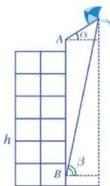
\includegraphics[width=0.3\textwidth]{img-1.jpeg}
    \end{center}
    \textcolor{book}{$\Rightarrow$} Đáp số: \dots\dots\dots\dots
    % Câu 3 (Gốc: B5)
    \item Cho đường tròn lượng giác có bán kính bằng 4 và góc $\alpha = \frac{4\pi}{3}$ như hình vẽ. Tính diện tích của hình thang $ABCD$ trong hình vẽ bên.
    
    \begin{center}
        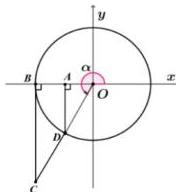
\includegraphics[width=0.3\textwidth]{img-6.jpeg}
    \end{center}
    \textcolor{book}{A.} $6\sqrt{2}$. \hspace{1.5cm} \textcolor{book}{B.} $3\sqrt{3}$. \hspace{1.5cm} \textcolor{book}{C.} $6\sqrt{3}$. \hspace{1.5cm} \textcolor{book}{D.} 6.
    % Câu 4 (Gốc: A4)
    \item Cho tam giác $ABC$ có ba cạnh $a = 5, b = 6, c = 7$. Tính $\cos A$.
    
    \textcolor{book}{A.} $\frac{5}{7}$. \hspace{1cm} \textcolor{book}{B.} $\frac{2}{21}$. \hspace{1cm} \textcolor{book}{C.} $\frac{55}{42}$. \hspace{1cm} \textcolor{book}{D.} $\frac{10}{7}$.
    % Câu 5 (Gốc: B12)
    \item Kim giờ dài 6 cm và kim phút dài 11 cm của đồng hồ chỉ 4 giờ. Hỏi thời gian ít nhất để 2 kim vuông góc với nhau là bao nhiêu? Lúc đó tổng quãng đường hai đầu mút kim giờ và kim phút đi được là bao nhiêu?
    
    \textcolor{book}{$\Rightarrow$} Đáp số: \dots\dots\dots\dots
    % Câu 6 (Gốc: A9)
    \item Trong một khu bảo tồn, người ta xây dựng một tháp canh và hai bồn chứa nước A, B để phòng hỏa hoạn. Từ tháp canh, người ta phát hiện đám cháy và số liệu đưa về như dưới. Nên dẫn nước từ bồn chứa A hay B để dập tắt đám cháy nhanh hơn?
    
    \begin{center}
        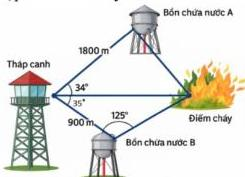
\includegraphics[width=0.5\textwidth]{img-3.jpeg}
    \end{center}
    \textcolor{book}{$\Rightarrow$} Đáp số: \dots\dots\dots\dots
    % Câu 7 (Gốc: B3)
    \item Đơn giản biểu thức $A = \cos\left(\frac{9\pi}{2} - \alpha\right) + \sin(\alpha - \pi)$ ta được
    
    \textcolor{book}{A.} $A = \cos \alpha + \sin \alpha$. \hspace{1cm} \textcolor{book}{B.} $A = 2 \sin \alpha$. \hspace{1cm} \textcolor{book}{C.} $A = \sin \alpha \cos \alpha$. \hspace{1cm} \textcolor{book}{D.} $A = 0$.
    % Câu 8 (Gốc: A2)
    \item Tìm khẳng định sai với các giá trị $x$ làm cho các biểu thức có nghĩa.
    
    \textcolor{book}{A.} $\sin(\pi - x) = \sin x$. \hspace{1.5cm} \textcolor{book}{B.} $\cos(\pi - x) = \cos x$. \\
    \textcolor{book}{C.} $\tan(\pi - x) = -\tan x$. \hspace{1.2cm} \textcolor{book}{D.} $\cot(\pi - x) = -\cot x$.
    % Câu 9 (Gốc: B8)
    \item Một vệ tinh được định vị tại vị trí $A$ trong không gian. Từ vị trí $A$, vệ tinh bắt đầu chuyển động quanh Trái Đất theo quỹ đạo là đường tròn với tâm $O$ của Trái Đất, bán kính 9 000 km. Biết rằng vệ tinh chuyển động hết một vòng của quỹ đạo trong 2 h.
    \begin{enumerate}
        \item Hãy tính quãng đường vệ tinh đã chuyển động được sau: 1h; 3h; 5h.
        \item Vệ tinh chuyển động được quãng đường 200 000 km sau bao nhiêu giờ (làm tròn đến kết quả hàng đơn vị)?
    \end{enumerate}
    \textcolor{book}{$\Rightarrow$} Đáp số: \dots\dots\dots\dots
    % Câu 10 (Gốc: A11)
    \item Hai người quan sát khinh khí cầu tại hai địa điểm P và Q nằm ở sườn đồi nghiêng 32° so với phương ngang, cách nhau 60 m. Người quan sát tại P xác định góc nâng của khinh khí cầu là 62°. Cùng lúc đó, người quan sát tại Q xác định góc nâng của khinh khí cầu đó là 70°. Tính khoảng cách từ Q đến khinh khí cầu.
    
    \begin{center}
        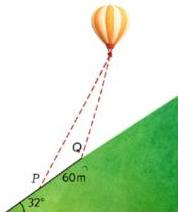
\includegraphics[width=0.4\textwidth]{img-5.jpeg}
    \end{center}
    \textcolor{book}{$\Rightarrow$} Đáp số: \dots\dots\dots\dots
    % Câu 11 (Gốc: B7)
    \item Một máy kéo nông nghiệp với bánh xe sau có đường kính là 184 cm, xe chuyển động với vận tốc không đổi trên một đoạn đường thẳng. Biết rằng vận tốc của bánh xe sau trong chuyển động này là 80 vòng/phút. Quãng đường mà xe đi được trong 10 phút được biểu diễn dưới dạng $a\pi$ (km). Giá trị của $a$ bằng bao nhiêu?
    
    \textcolor{book}{$\Rightarrow$} Đáp số: \dots\dots\dots\dots
\end{enumerate}
\end{document}